\documentclass[10.5pt]{report}
\usepackage[a4paper,margin=0.9in]{geometry}
\usepackage{amsmath,amssymb}
\usepackage{booktabs}
\usepackage{graphicx}
\usepackage[colorlinks=true,linkcolor=blue]{hyperref}
\usepackage{xcolor}
\usepackage{titlesec}
\usepackage{caption}
\definecolor{hbblue}{HTML}{2A4D8F}
\titleformat{\chapter}[display]{\bfseries\Large\color{hbblue}}{\chaptertitlename\ \thechapter}{6pt}{\Large}
\captionsetup{font=small,labelfont=bf}

\title{\textbf{\Large Blur-Optimum vs.\ Acuity-Optimum Aperture}\\[0.2cm]
\textcolor{hbblue}{\large Mapped Individually at Each Myopia Level}\\[0.3cm]
\normalsize\itshape Same fresh, corrected-optics data as
\texttt{Fresh\_Sweep\_Analysis.pdf} (\texttt{new\_sweeps/blur\_sweep.csv},
\texttt{acuity\_sweep\_stage4.csv}) --- no new sweep run, replotted per myopia level.}
\author{}
\date{}

\begin{document}
\maketitle
\tableofcontents

\chapter{What this document shows}

\texttt{Fresh\_Sweep\_Analysis.pdf} showed the blur-optimal and acuity-optimal
aperture \emph{as a function of} myopia $M$ on one summary chart (its Figure~4).
This document instead maps, \textbf{individually for each tested myopia level},
exactly where each optimum sits on its own full curve --- the blur curve
($r_{EE}(50\%)$ at the retina) and the acuity curve (predicted logMAR), aperture on
the $x$-axis, with a star marking the minimum and a dashed guide line at each
optimum's aperture so the gap between the two is visible directly, not just as a
single number in a table.

\textbf{Grid}: the same 15 apertures $\times$ 8 myopia levels
($M\in\{0,1,2,3,4,5,6,8\}$D) as \texttt{Fresh\_Sweep\_Analysis.pdf}, same corrected
optics (\texttt{stage2\_fixed/}), same acuity model (\texttt{stage4\_human\_vision}'s
recommended predictor). No aperture recommendation is made anywhere below.

\section{Summary table}

\begin{table}[htbp]
\centering
\begin{tabular}{rrrrrr}
\toprule
$M$ (D) & Blur-optimal ($\mu$m) & $r_{EE}(50\%)$ there & Acuity-optimal ($\mu$m) & logMAR there & Gap \\
\midrule
0 & 700 & 7.33$^{\ast}$  & 2000$^{\dagger}$ & $-$0.344 & +185.7\% \\
1 & 700 & 7.33$^{\ast}$  & 1250  & $-$0.120 & +78.6\% \\
2 & 750 & 8.01  & 750  & 0.076 & 0.0\% \\
3 & 600 & 10.57 & 750  & 0.112 & +25.0\% \\
4 & 500 & 12.02 & 600  & 0.181 & +20.0\% \\
5 & 500 & 13.29 & 600  & 0.240 & +20.0\% \\
6 & 400 & 14.47 & 500  & 0.259 & +25.0\% \\
8 & 400 & 17.87 & 400  & 0.331 & 0.0\% \\
\bottomrule
\end{tabular}
\caption{$^{\ast}$Inside the $r_{EE}(50\%)$ histogram bin-width floor
(\texttt{Fresh\_Sweep\_Analysis.pdf}, Ch.~2) --- lower-confidence. $^{\dagger}$Boundary
artifact, not a genuine interior minimum --- see the note below and
Figure~\ref{fig:M0}. Gap = (acuity-optimal $-$ blur-optimal)/blur-optimal.}
\end{table}

\textbf{A caveat found while building this document, stated plainly}: at $M=0$D
specifically, the acuity (logMAR) curve is still monotonically \emph{decreasing} at
the largest tested aperture (2000\,$\mu$m, Figure~\ref{fig:M0}) --- it never turns
back up within the tested range. The reported ``acuity-optimal: 2000\,$\mu$m'' at
$M=0$D is therefore the \emph{edge of the tested aperture range}, not a genuine
interior minimum, and the true acuity optimum at $M=0$D may lie beyond 2000\,$\mu$m
(untested here). This was checked directly, not assumed: every other myopia level
($M\ge1$D, Figures~\ref{fig:M1}--\ref{fig:M8}) shows the acuity curve turning back up
well inside the tested range, a genuine interior minimum. $M=1$D's acuity curve turns
around at 1250\,$\mu$m, comfortably inside the 2000\,$\mu$m ceiling, so only the
$M=0$D row above should be treated as boundary-limited.

\chapter{Individual myopia-level maps}

\begin{figure}[htbp]
\centering
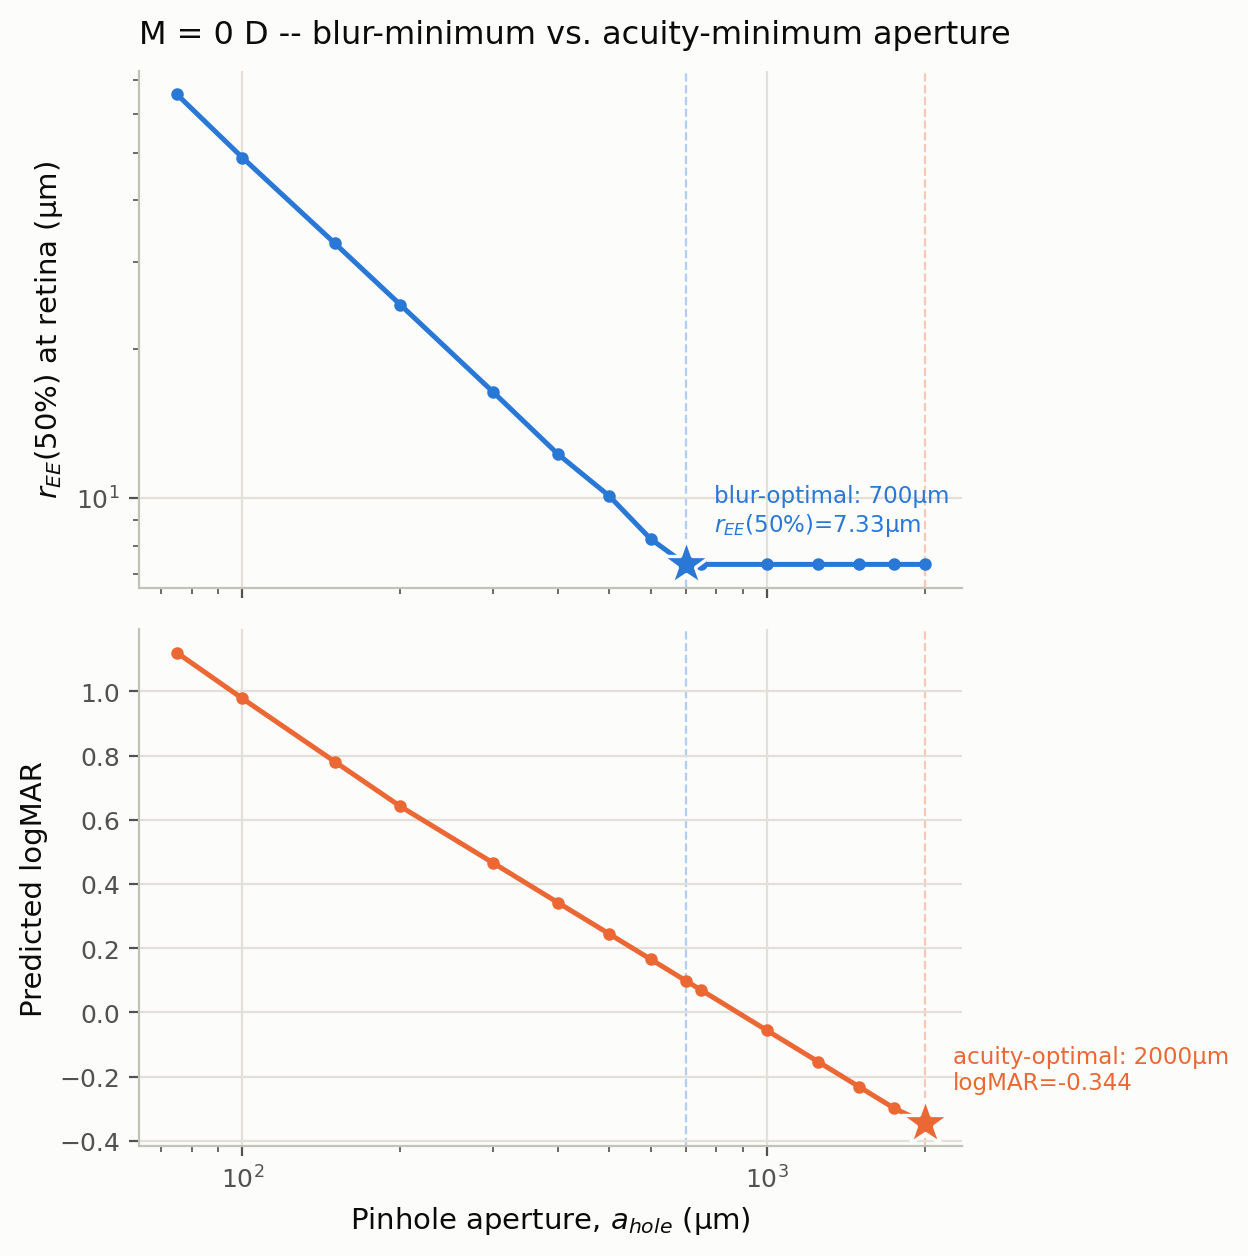
\includegraphics[width=0.8\textwidth]{figures/fig_M0.png}
\caption{$M=0$D (emmetropic baseline). See the boundary-artifact note above --- the
acuity curve has not yet turned back up by 2000\,$\mu$m.}
\label{fig:M0}
\end{figure}

\begin{figure}[htbp]
\centering
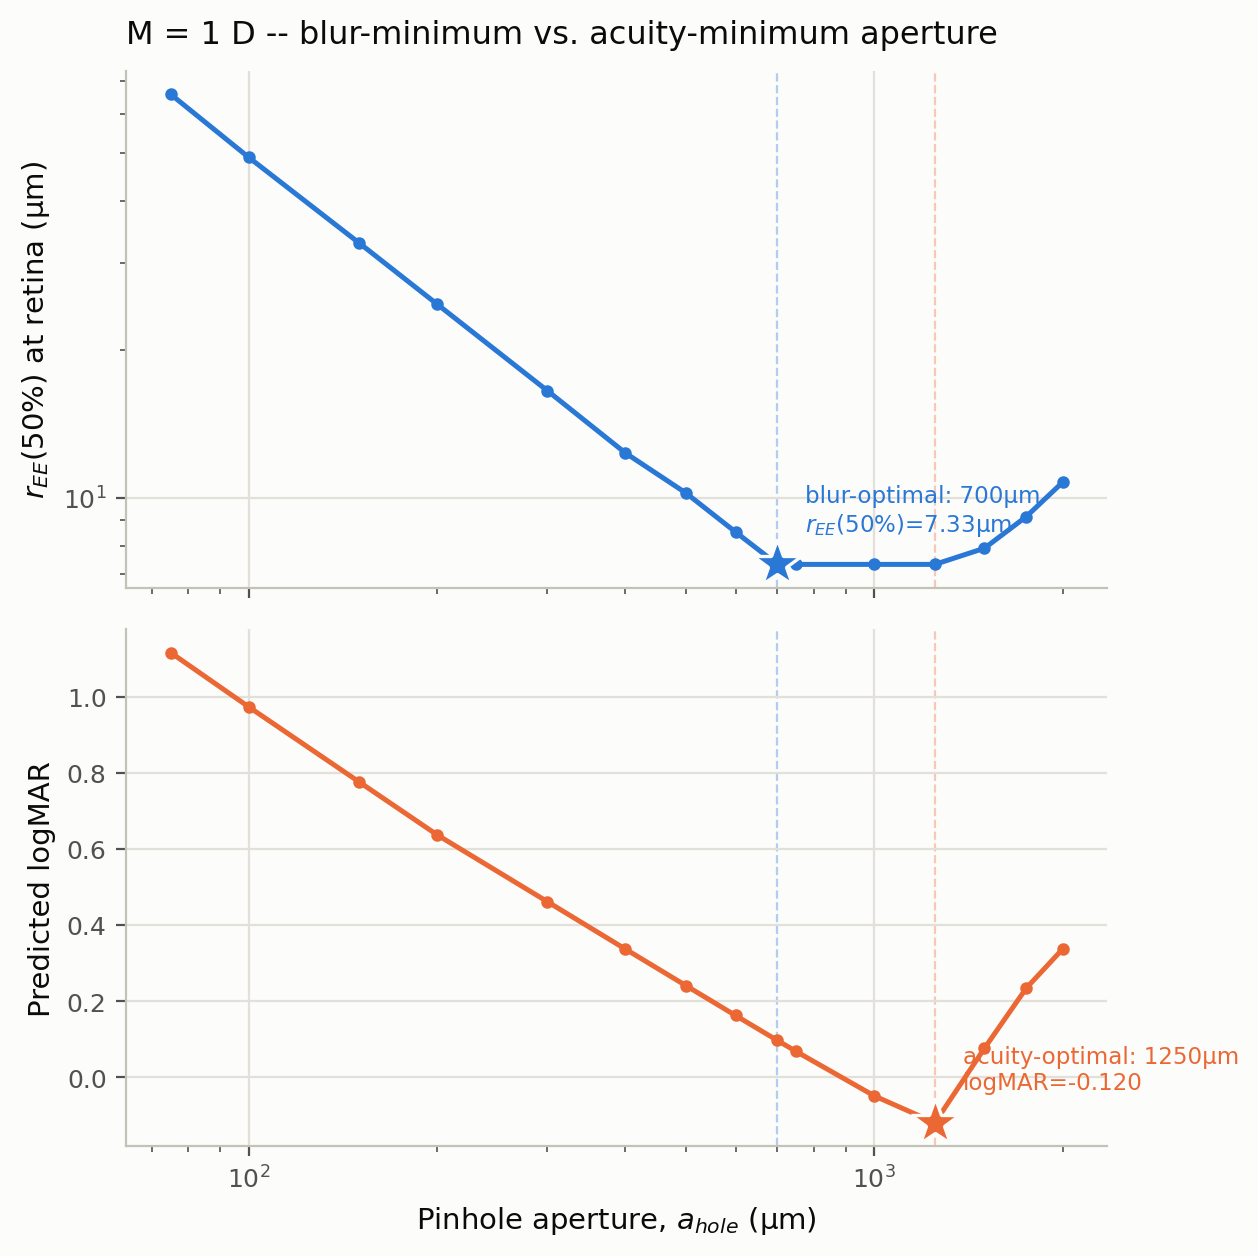
\includegraphics[width=0.8\textwidth]{figures/fig_M1.png}
\caption{$M=1$D. Both curves show a genuine interior minimum.}
\label{fig:M1}
\end{figure}

\begin{figure}[htbp]
\centering
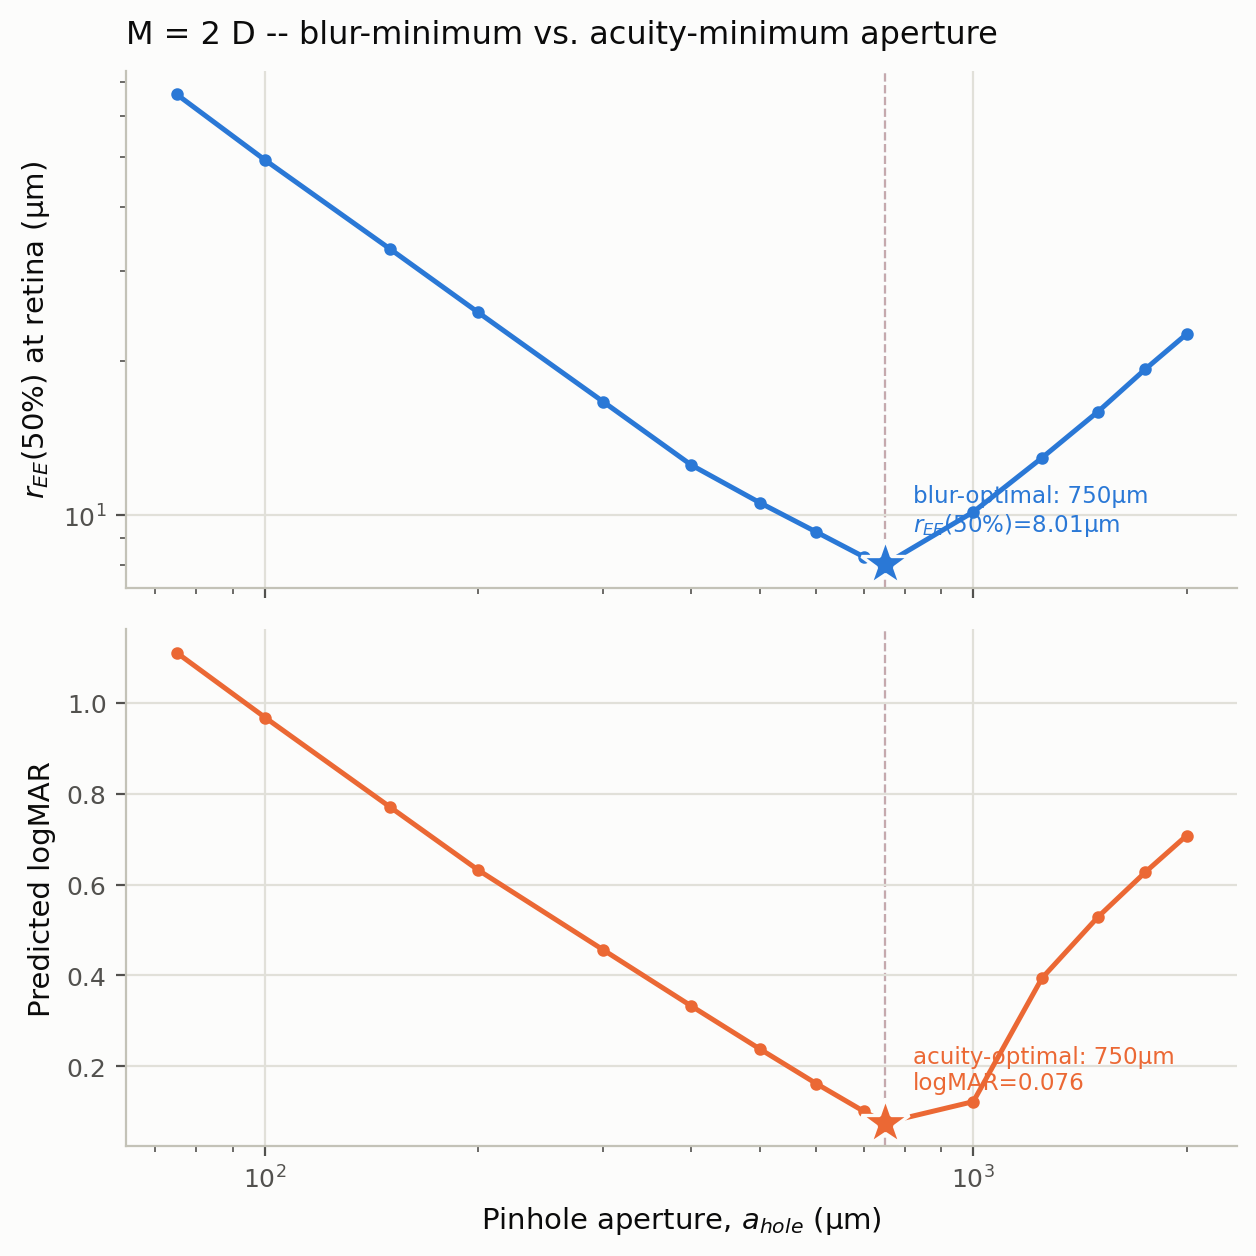
\includegraphics[width=0.8\textwidth]{figures/fig_M2.png}
\caption{$M=2$D. Blur-optimal and acuity-optimal coincide exactly (750\,$\mu$m).}
\label{fig:M2}
\end{figure}

\begin{figure}[htbp]
\centering
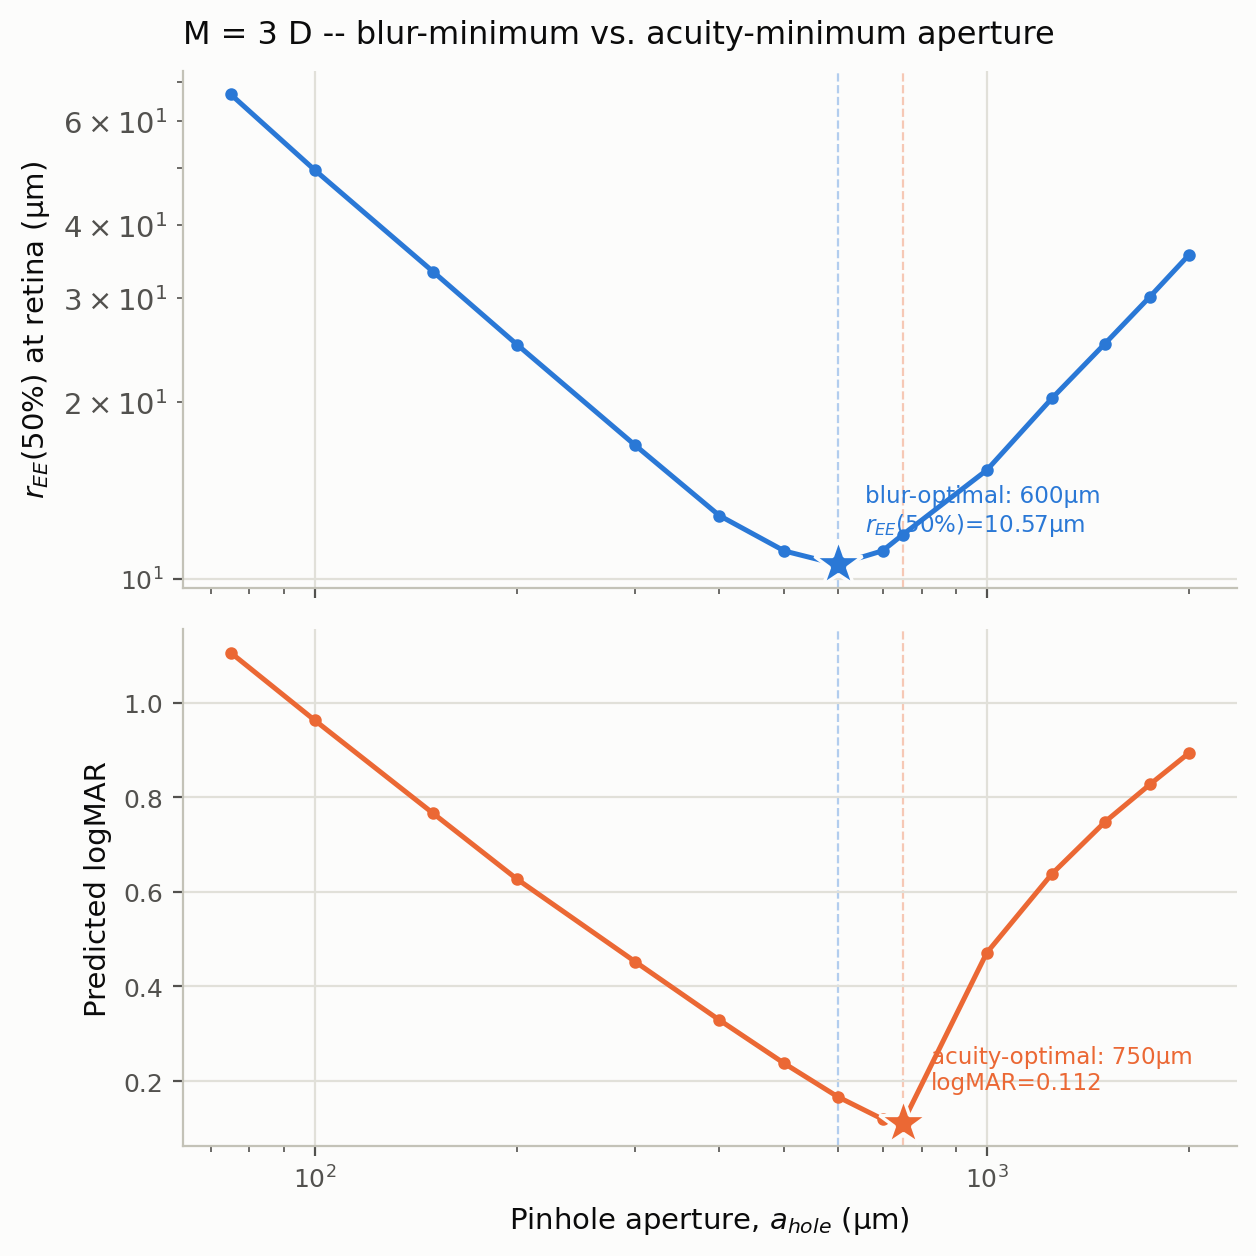
\includegraphics[width=0.8\textwidth]{figures/fig_M3.png}
\caption{$M=3$D.}
\label{fig:M3}
\end{figure}

\begin{figure}[htbp]
\centering
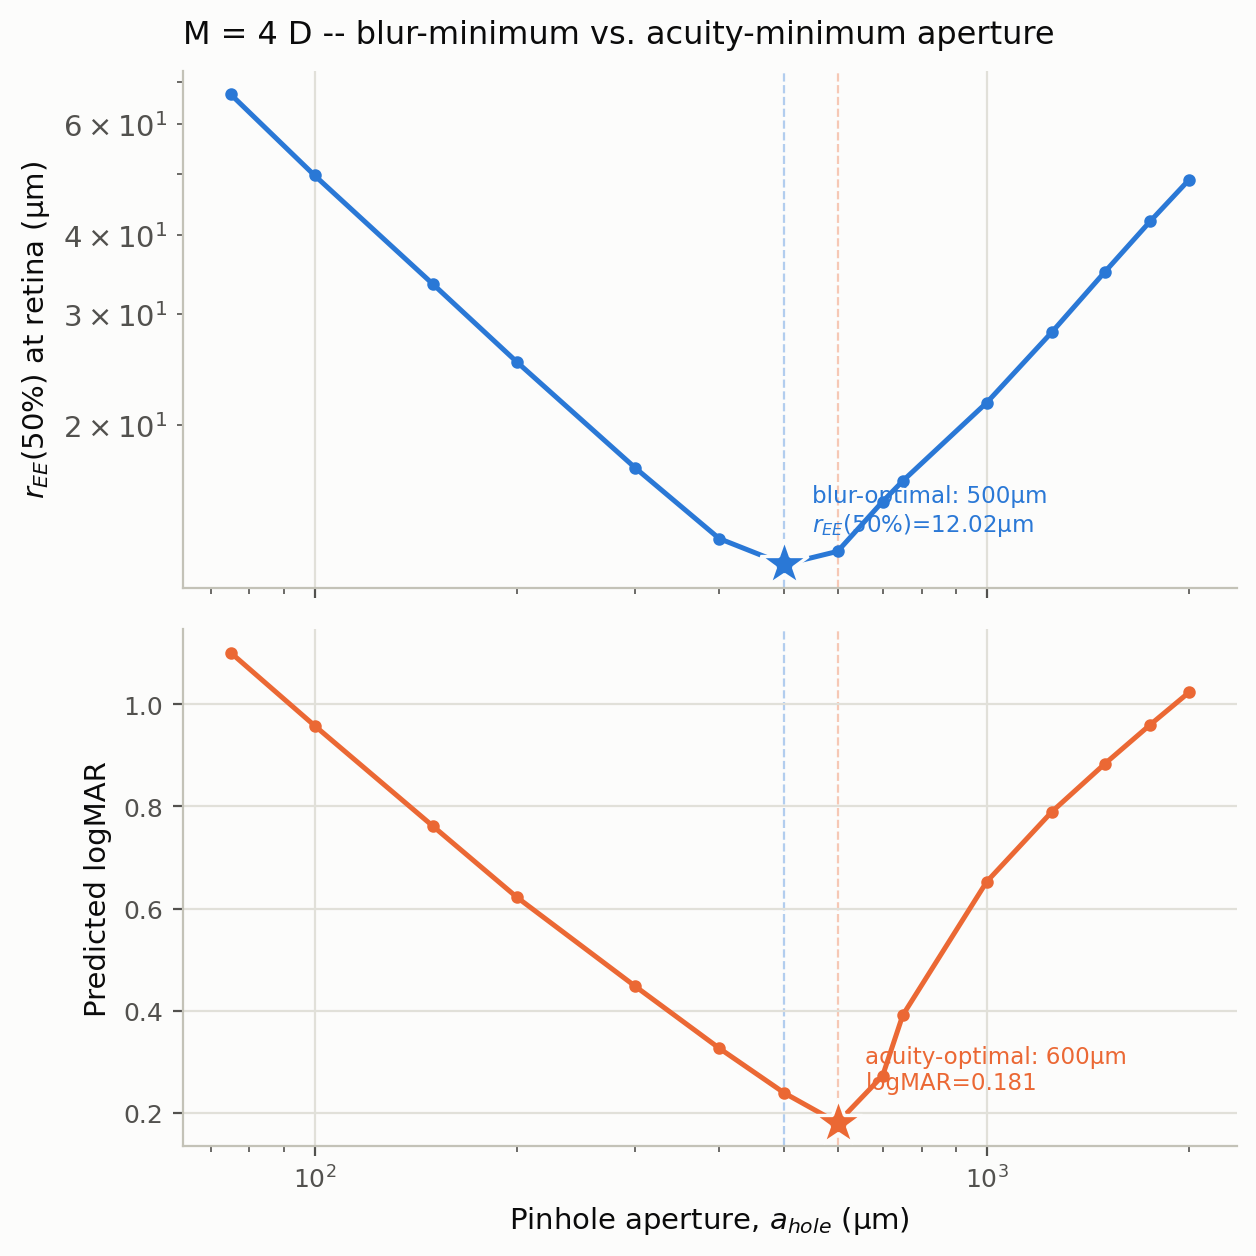
\includegraphics[width=0.8\textwidth]{figures/fig_M4.png}
\caption{$M=4$D.}
\label{fig:M4}
\end{figure}

\begin{figure}[htbp]
\centering
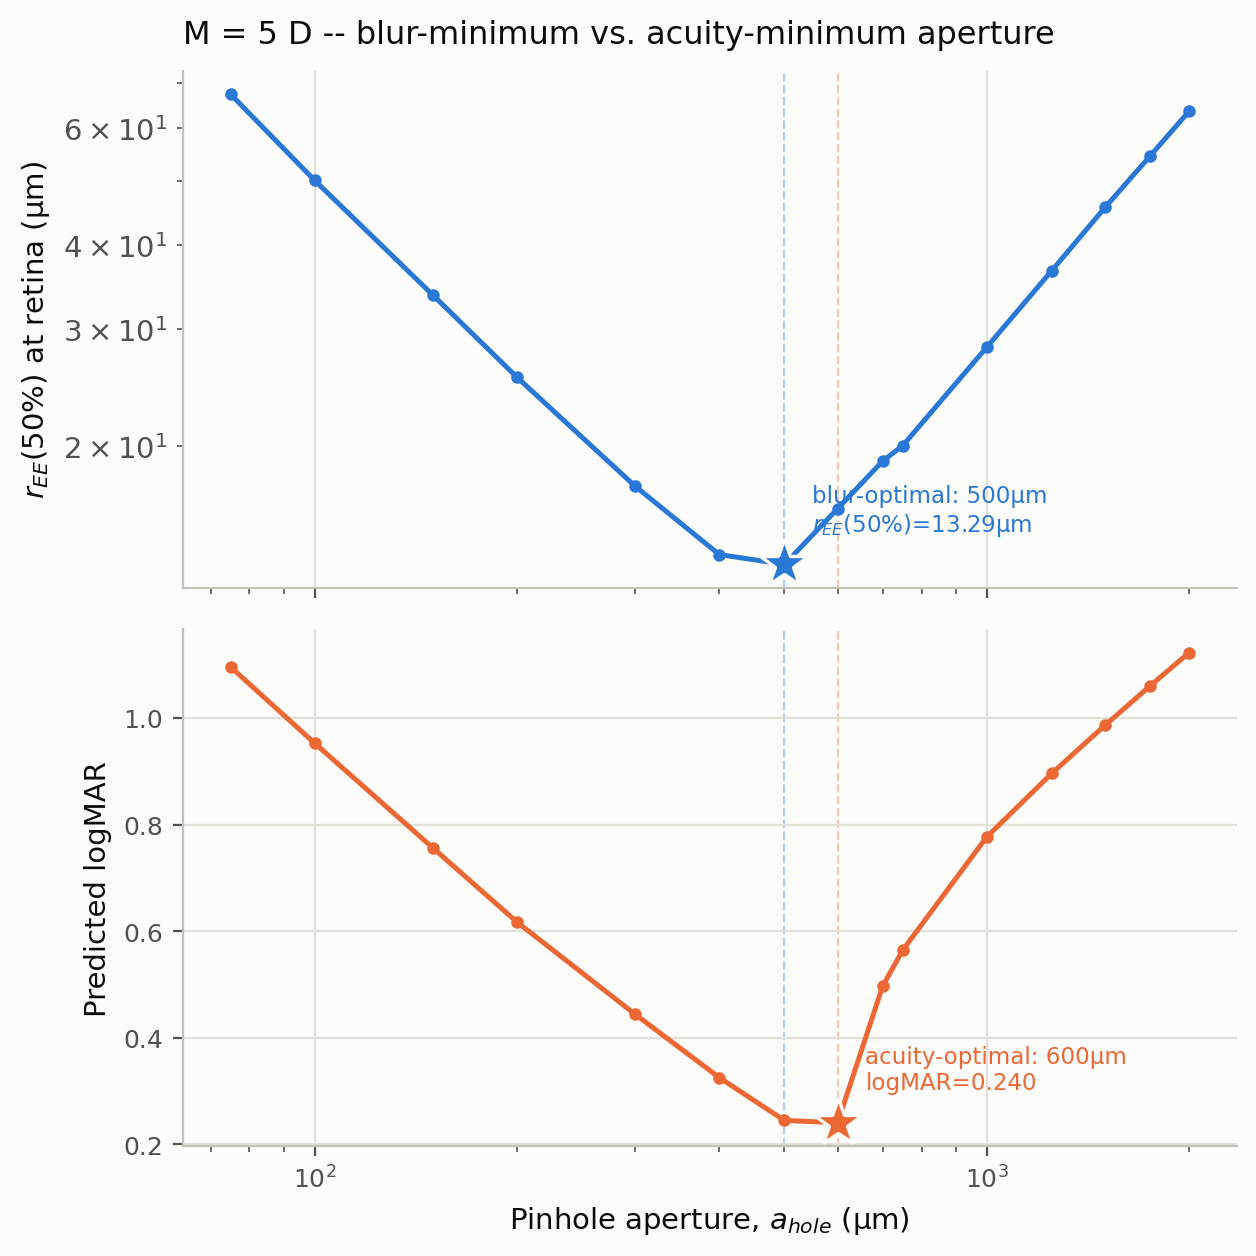
\includegraphics[width=0.8\textwidth]{figures/fig_M5.png}
\caption{$M=5$D.}
\label{fig:M5}
\end{figure}

\begin{figure}[htbp]
\centering
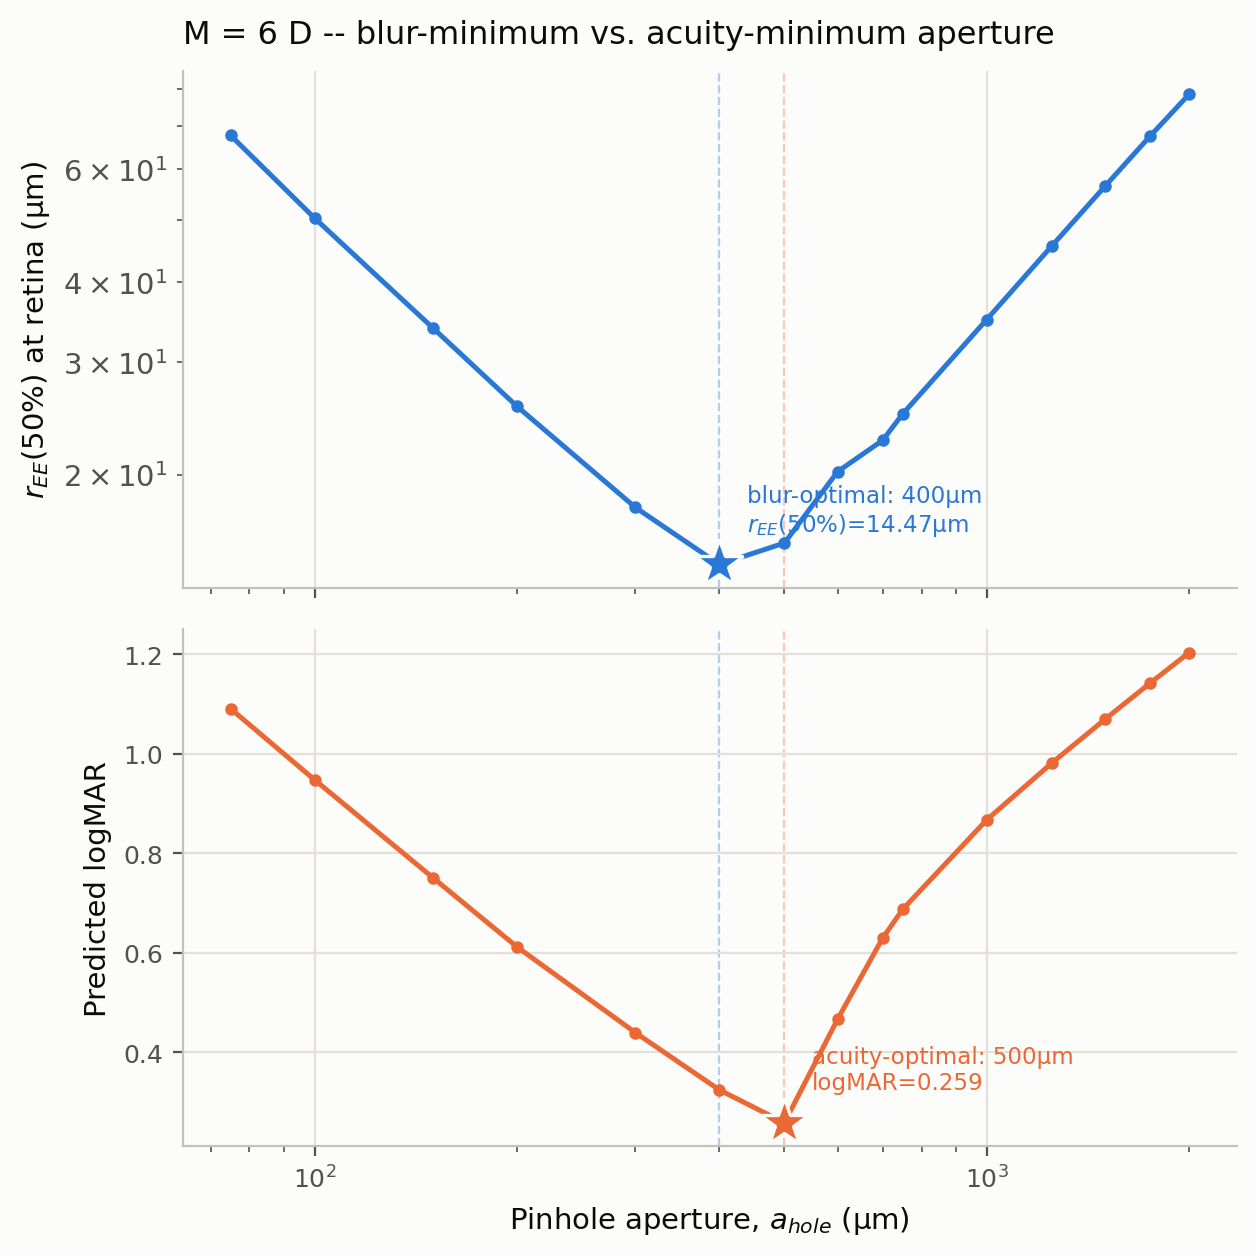
\includegraphics[width=0.8\textwidth]{figures/fig_M6.png}
\caption{$M=6$D.}
\label{fig:M6}
\end{figure}

\begin{figure}[htbp]
\centering
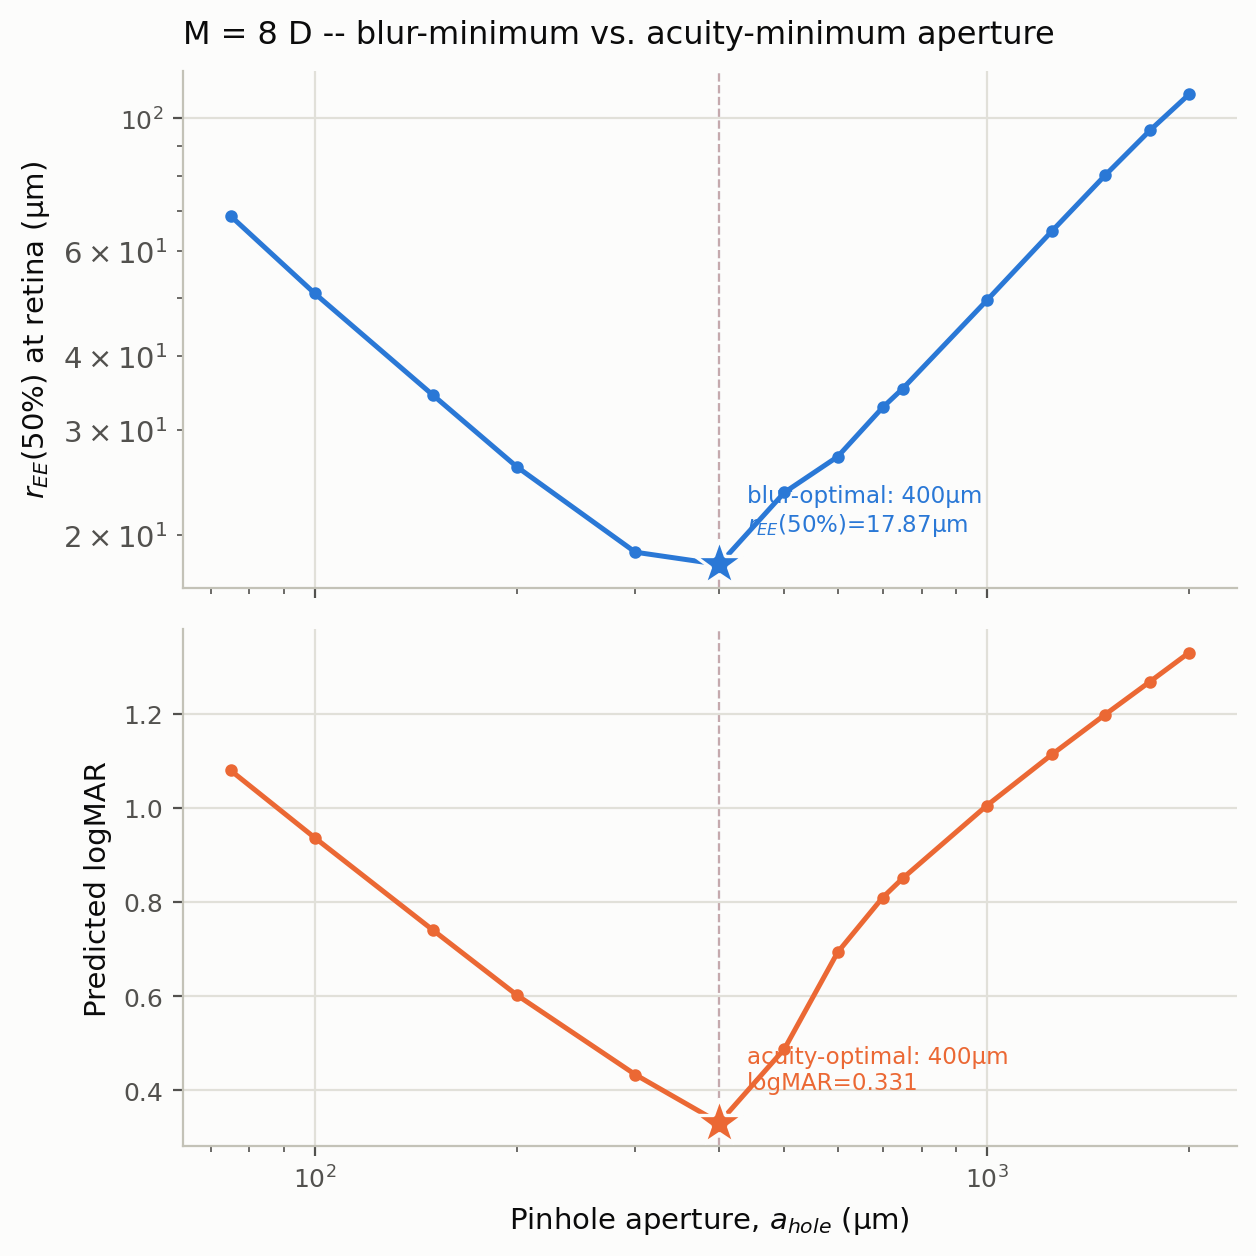
\includegraphics[width=0.8\textwidth]{figures/fig_M8.png}
\caption{$M=8$D (highest myopia tested). Blur-optimal and acuity-optimal coincide
exactly (400\,$\mu$m).}
\label{fig:M8}
\end{figure}

\chapter{Reading across the maps}

The gap between the two optima shrinks from +185.7\% at $M=0$D (caveated above) to
exactly 0\% at $M=8$D, and the two curves visibly converge in shape as $M$ increases
(Figures~\ref{fig:M1}--\ref{fig:M8}): at low myopia the acuity curve's minimum is far
broader and shifted well to the right of the blur curve's minimum, while at high
myopia the two minima sit directly on top of each other. This is consistent with
defocus blur increasingly dominating both metrics at high $M$ (both models are then
responding to the same effect), while at low $M$ the acuity model's additional
illuminance/contrast term still has room to reward a larger aperture that pure blur
minimization does not. No aperture recommendation is made anywhere in this document.

\end{document}
